% Intended LaTeX compiler: pdflatex
\documentclass[10pt,a4paper,UTF8]{article}
\usepackage{zclorg}
\usepackage{tikztheorem}
\author{zcl.space}
\date{}
\title{Functions and Maps}
\hypersetup{
 pdfauthor={zcl.space},
 pdftitle={Functions and Maps},
 pdfkeywords={PMA},
 pdfsubject={},
 pdfcreator={Emacs 25.0.50.1 (Org mode 9.1.2)},
 pdflang={English}}
\begin{document}

\maketitle
\tableofcontents
\titlepic{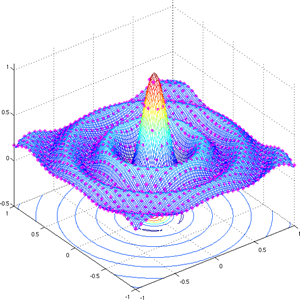
\includegraphics[scale=0.25]{../../img/sinc.PNG}}
 A \texttt{function} is a rule which assigns a value
\(f(x)\) to every point \(x\) from a set called the \texttt{domain} of the function.
The set
$$
  \mathrm{graph}(f):=\{(x,y): y=f(x)\}
$$
of all pairs \((x,y)\) such that \(y=f(x)\) is called the \texttt{graph} of the function \(f\).
Two functions are equal iff they have the same graph.

Let \(X\) and \(Y\) be sets.
We say that \(f\) is a \texttt{map}  from \(X\) to \(Y\)
and  write \(f:X\to Y\) when \(f\) is a function which assigns
a point \(y=f(x)\in Y\) to each point \(x\in X\).
Two maps \(f:X\to Y\) and \(f':X'\to Y'\) are
said to be \texttt{equal}
when \(X=X'\), \(Y=Y'\), and \(f(x)=f'(x)\) for all \(x\in X\).
Thus if \(f\) and \(f'\) equal maps, then \(\mathrm{graph}(f)=\mathrm{graph}(f')\)
but not conversely (because \(Y=Y'\) is part of the definition of equality for maps).
However most authors would say that two functions are equal iff they have the same graph.

 Some authors
use the notation \(x\mapsto f(x)\)
to define a map. This allows them to avoid introducing a name for the map. Thus instead of writing
\begin{quote}
Consider the map \(f:\mathbf{R}\to \mathbf{R}\) defined by \(f(x)=x^5+x\).
\end{quote}

they may write
\begin{quote}
Consider the map \(\mathbf{R}\to \mathbf{R}:x\mapsto x^5+x\).
\end{quote}

When \(A\subseteq X\), \(B\subseteq Y\), and \(f:X\to Y\), the sets

\begin{aligned}
  & f(A):=\{y\in Y: \exists x\in A \mbox{ such that }y=f(x)\}, \\
  & f^{-1}(B):=\{x\in X: f(x)\in B\},
\end{aligned}

are called respectively the \texttt{image} of \(A\)  by \(f\)
and  \texttt{inverse image}  of \(B\) by \(f\).

The sets \(X\)  and \(Y\) are sometimes called the
\texttt{source} and \texttt{target} of a map \(f:X\to Y\).
The image \(f(X)\) of the source is what is called the \{range\}
of the function \(f\) in calculus.
Thus the domain of a map is the same as its source
while the range is a subset of its target.

There are slight variations in terminology among  authors.
Morgan avoids the word \texttt{map} and Lang sometimes
uses the word \texttt{mapping}.  Buck uses the term the \texttt{preimage}
instead of \texttt{inverse image}. Lang  uses the \(\mapsto\)
notation but the other authors apparently avoid it.
For Lang a function is a map whose target is \(\mathbf{R}\).
In precalculus courses a function is usually defined by an expression
and the domain is implicitly taken to be the largest set of numbers
for which the expression is meaningful, but in advanced mathematics
authors usually make the domain explicit.
\end{document}
